\section{Ejercicio 7 - Definir cálculos}  

1. Abra el Diseñador de cubos y, a continuación, haga clic en la pestaña Cálculos
Observe el comando predeterminado CALCULATE en el panel de las expresiones de cálculo y en el panel
Organizador de scripts. Este comando especifica que las medidas del cubo deberían agregarse según el valor
especificado por sus propiedades AggregateFunction. Los valores de medida normalmente se suman, pero
también pueden contarse o agregarse de otra forma.

	\begin{center}
	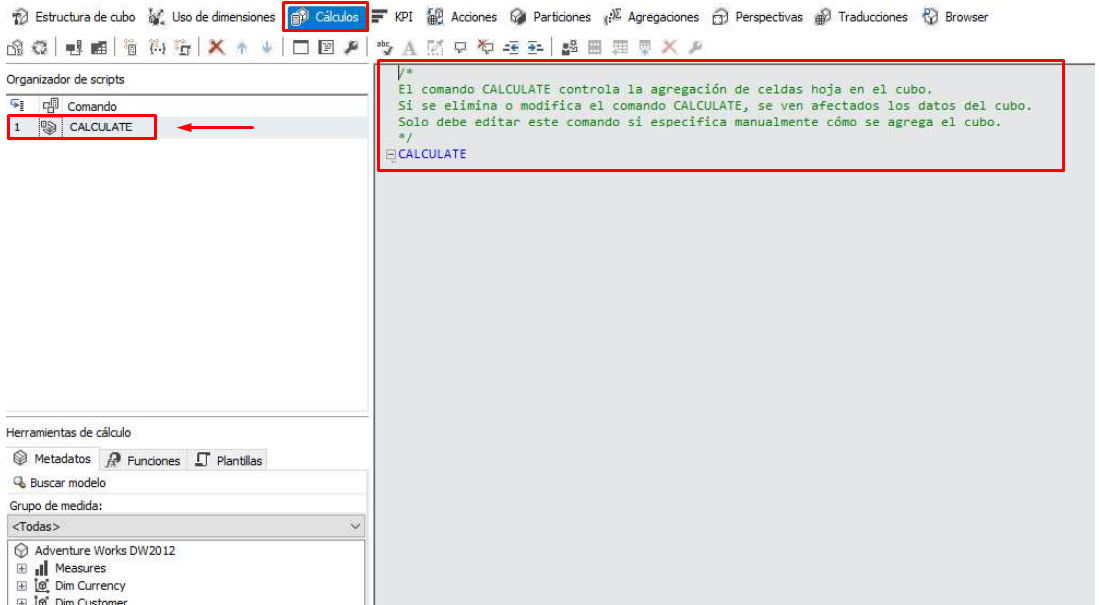
\includegraphics[width=\columnwidth]{images/task7/img1}
	\end{center}	

2. En la barra de herramientas de la pestaña Cálculos, haga clic en Nuevo miembro calculado
En el panel de las expresiones de cálculo aparece un nuevo formulario en el que podrá definir las propiedades de
este nuevo miembro calculado. El nuevo miembro aparecerá también en el panel Organizador de scripts. La siguiente imagen muestra el formulario que aparece en el panel de las expresiones de cálculo al hacer clic en Nuevo miembro calculado

	\begin{center}
	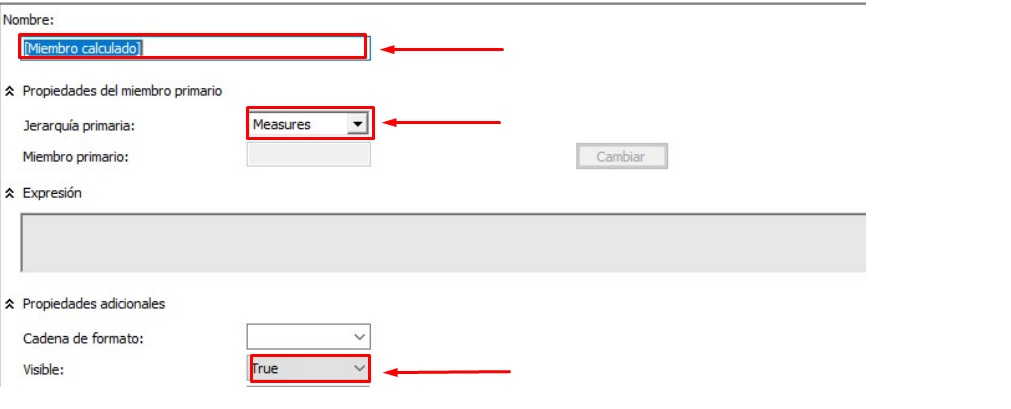
\includegraphics[width=\columnwidth]{images/task7/img2}
	\end{center}	

3. En el cuadro Nombre, cambie el nombre de la medida calculada por [Total de Ventas].
Si el nombre de un miembro calculado contiene un espacio, dicho nombre deberá ir entre corchetes.
Observe que en la lista Jerarquía primaria, de manera predeterminada, se crea un nuevo miembro calculado en
la dimensión Measures. A un miembro calculado de la dimensión Measures también se le denomina con
frecuencia medida calculada.

4. En la pestaña Metadatos del panel Herramientas de cálculo

	\begin{center}
	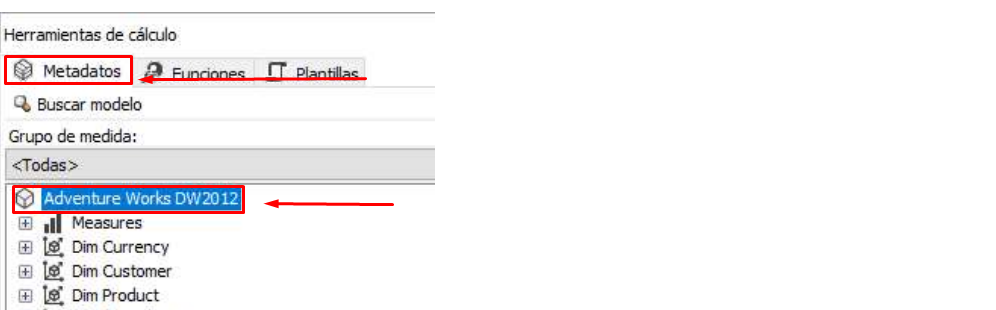
\includegraphics[width=\columnwidth]{images/task7/img3}
	\end{center}	

5.Expanda Medidas (Measures) y, a continuación, FactInternet Sales para ver los metadatos del grupo de medida
FactInternet Sales.

	\begin{center}
	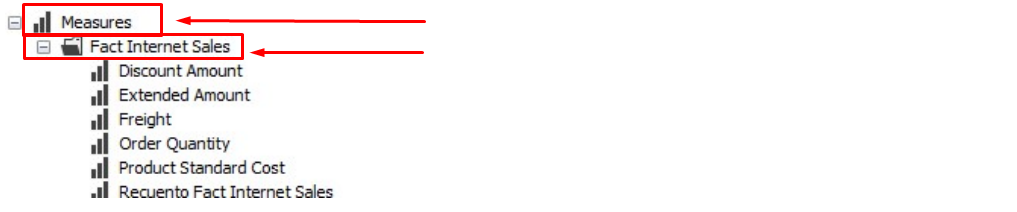
\includegraphics[width=\columnwidth]{images/task7/img4}
	\end{center}	

Puede arrastrar los elementos de metadatos desde el panel Herramientas de cálculo al cuadro Expresión y
agregar entonces operadores y otros elementos para crear expresiones multidimensionales (MDX). O bien, puede
escribir la expresión MDX directamente en el cuadro Expresión

	\begin{center}
	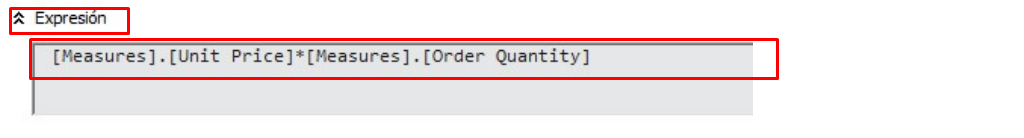
\includegraphics[width=\columnwidth]{images/task7/img5}
	\end{center}	

6. En la lista Cadena de formato, seleccione "Currency"

7. En la lista Comportamiento si no está vacío, active las casillas de verificación Unit Price y haga clic en Aceptar.

	\begin{center}
	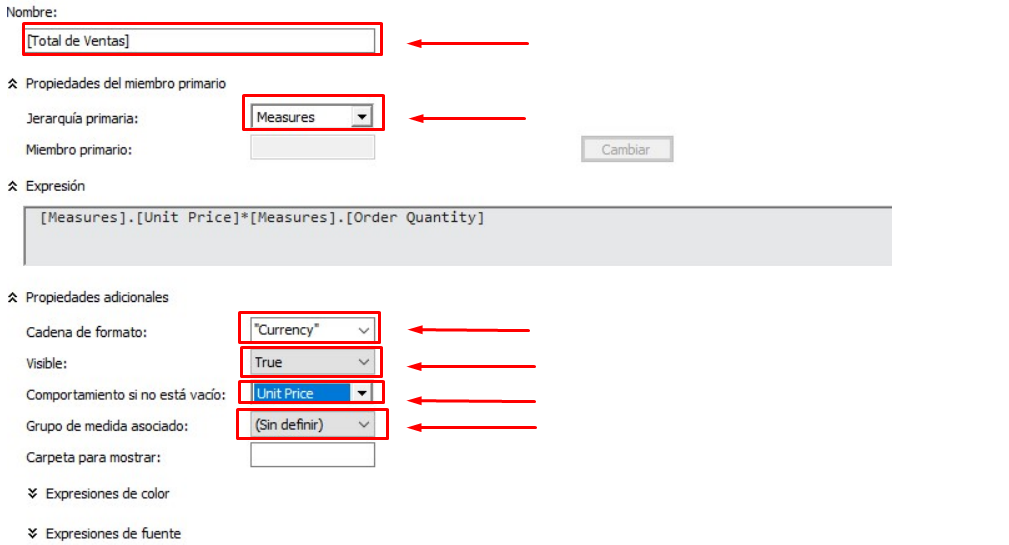
\includegraphics[width=\columnwidth]{images/task7/img6}
	\end{center}	

Las medidas especificadas en la lista Comportamiento si no está vacío se utilizan para resolver consultas NON
EMPTY en MDX. Si se especifican una o más medidas en la lista Comportamiento si no está vacío, Analysis Services
tratará al miembro calculado como vacío si todas las medidas especificadas están vacías. Si la propiedad Nonempty behavior está en blanco, Analysis Services deberá evaluar al miembro calculado para determinar si el
miembro está vacío.

8. En la barra de herramientas de la pestaña Cálculos, haga clic en Vista de script y revise la script del cálculo
en el panel de las expresiones de cálculo.

	\begin{center}
	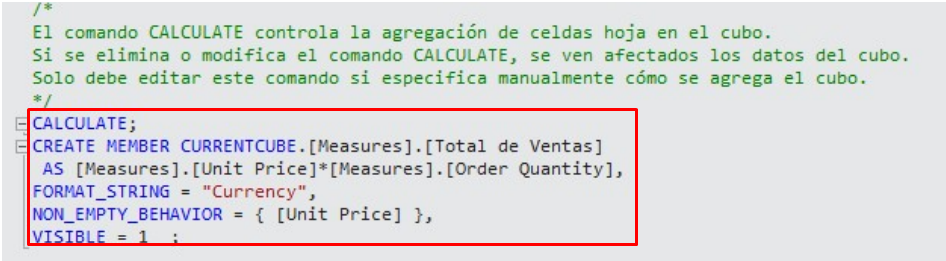
\includegraphics[width=\columnwidth]{images/task7/img7}
	\end{center}	

Observe que el nuevo cálculo se agrega a la expresión CALCULATE inicial; los cálculos individuales se separan con
un punto y coma. Observe también que aparece un comentario al principio de la script del cálculo. Se recomienda
la agregación de comentarios dentro de la script de cálculo para grupos de cálculos para ayudarle a usted y a otros
programadores a comprender las scripts de cálculo complejas.

9. Guardar los cambios

10. Cerrar el diseñador del cubo

11. Procesar el cubo

12. Examinar el cubo

13. Abrir el diseñador del Cubo y en la pestaña Cálculos en la opción de Grupo de medida observe el nuevo miembro
calculado

	\begin{center}
	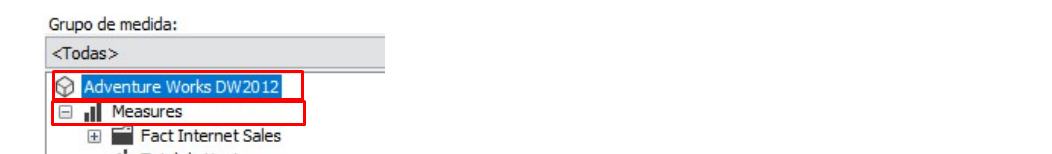
\includegraphics[width=\columnwidth]{images/task7/img8}
	\end{center}	

\subsection{Definir cálculos de margen de beneficio bruto}  

1. Haga clic en Nuevo miembro calculado en la barra de herramientas de la pestaña Cálculos. 

2. En el cuadro Nombre, cambie el nombre de esta nueva medida calculada por [Porcentaje Costo Producto].

3. En el cuadro Expresión, cree la siguiente expresión MDX:

[Measures].[Total Product Cost]/[Measures].[Sales Amount]

4. Verifique las propiedades adicionales, así como se muestra en la siguiente imagen

	\begin{center}
	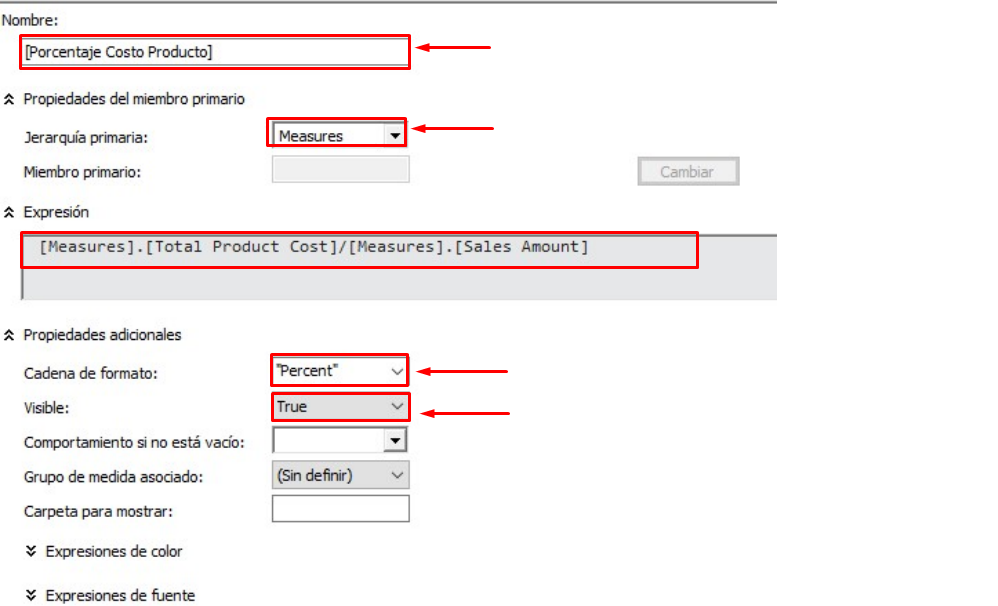
\includegraphics[width=\columnwidth]{images/task7/img9}
	\end{center}	


5. Guardar los cambios al proyecto

6. Cerrar el diseñador del cubo

7. Procesar el cubo

8. Examinar el cubo

9. Abrir el diseñador del Cubo y en la pestaña Cálculos en la opción de Grupo de medida observe el nuevo miembro
calculado

	\begin{center}
	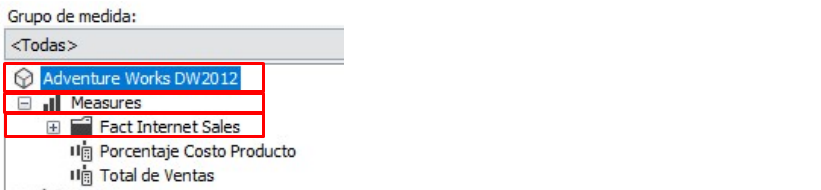
\includegraphics[width=\columnwidth]{images/task7/img10}
	\end{center}	


La siguiente imagen muestra el panel Script View con los cálculos creados.

	\begin{center}
	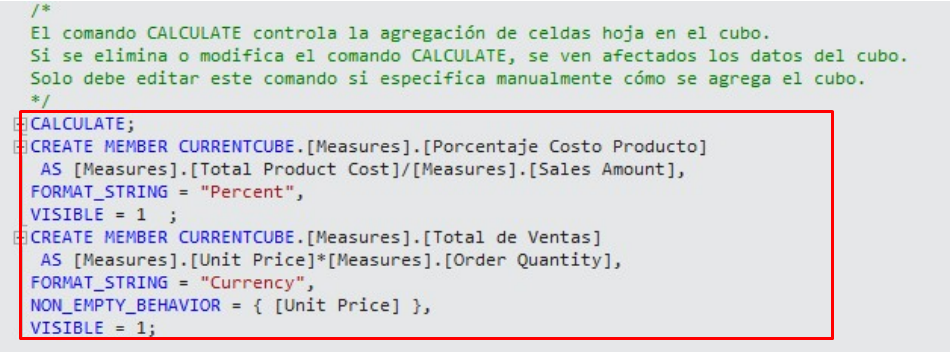
\includegraphics[width=\columnwidth]{images/task7/img11}
	\end{center}	


\subsection{Examinar los nuevos miembros calculados}  

1. Hacer clic en la pestaña Browser

2. Arrastrar los nuevos campos calculados para verificar su funcionamiento, así como se muestra a continuación:

	\begin{center}
	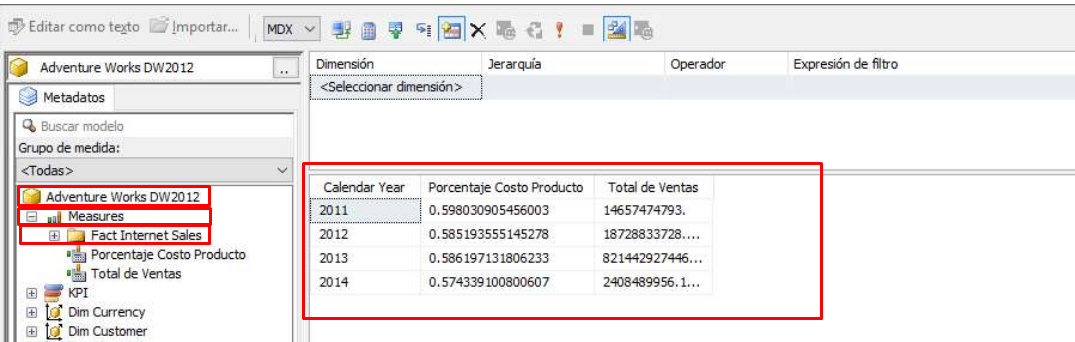
\includegraphics[width=\columnwidth]{images/task7/img12}
	\end{center}	
